% !TEX root = ../../../main.tex

\toggletrue{image}
\toggletrue{imagehover}
\chapterimage{x}
\chapterimagetitle{\uppercase{X}}
\chapterimageurl{https://xkcd.com/2309/}
\chapterimagehover{The worst is when you run out of monospaced fonts and have to use variable-width variables.}

\chapter{Variablen}
\label{chapter-variablen}

Für einfachere und vielseitigere Programme müssen wir in der Lage sein, eine Zahl oder einen Text zu speichern. In den Programmiersprachen stehen dafür \textbf{benannte Speicherplätze} zur Verfügung. Das Speichern von z.B. Zahlen oder Text dürfen wir nicht mit dem Speichern z.B. eines Textdokuments verwechseln. Ein Speicherplatz ist nur während das Programm läuft verfügbar. Danach sind alle Speicherplätze wieder gelöscht. Die Lernziele für dieses Kapitel sind:

\newcommand{\variablenLernziele}{
\protect\begin{todolist}
\item Sie definieren die Begriffe Variable, Wert, Literal und Zuweisung.
\item Sie verwenden Variablen, um Python-Programme einfacher und vielseitiger zu gestalten.
\item Sie wissen, welche Variablennamen in Python erlaubt sind.
\item Sie berücksichtigen die Clean-Code-Regeln im Umgang mit Variablen.
\end{todolist}
}

\lernziel{\autoref{chapter-variablen}, \nameref{chapter-variablen}}{\protect\variablenLernziele}

\variablenLernziele

\section{Quadrate mit unterschiedlicher Länge}

Schauen wir uns das Programm aus \autoref{lst-quadrat-100} an, welches ein Quadrat mit der Seitenlänge $100$ zeichnet. Wenn wir nun ein Quadrat mit der Seitenlänge $275$ zeichnen möchten, dann müssen wir das Programm an \textbf{vier} Stellen anpassen. \autoref{lst-quadrat-275} zeigt das angepasste Programm. Optimal wäre das Programm, wenn wir es nur an \textbf{einer} Stelle anpassen müssten. Dies können wir erreichen, in dem wir eine \textbf{Variable} verwenden. 

\begin{figure}[htb]
\centering
\begin{minipage}{0.4\linewidth}
\centering
\begin{lstlisting}[caption={Quadrat (Länge $100$).}, label=lst-quadrat-100]
import turtle

turtle.fd(100)
turtle.lt(90)
turtle.fd(100)
turtle.lt(90)
turtle.fd(100)
turtle.lt(90)
turtle.fd(100)
turtle.lt(90)
turtle.done()
\end{lstlisting}
\end{minipage}
\hfill
\begin{minipage}{0.4\linewidth}
\centering
\begin{lstlisting}[caption={Quadrat (Länge $275$).}, label=lst-quadrat-275]
import turtle

turtle.fd(275)
turtle.lt(90)
turtle.fd(275)
turtle.lt(90)
turtle.fd(275)
turtle.lt(90)
turtle.fd(275)
turtle.lt(90)
turtle.done()
\end{lstlisting}
\end{minipage}
\end{figure}

Wir speichern die Zahl für die Seitenlänge des Quadrats in einer Variablen ab und verwenden die Variable anschliessend als Argument bei den vier Funktionsaufrufen. \autoref{lst-quadrat-var-100} zeigt das verbesserte Programm. Wenn das Programm ausgeführt wird, dann wird in Zeile \textbf{drei} die Zahl $100$ in der Variablen mit dem Namen \lstinline{a} gespeichert. In den Zeilen vier, sechs, acht und zehn wird die Variable \lstinline{a} dann durch die gespeicherte Zahl ersetzt.

\begin{figure}[htb]
\centering
\begin{minipage}{0.4\linewidth}
\centering
\begin{lstlisting}[caption={Die Variable \lstinline{a} speichert die Zahl $100$ (\graybgtexttt{quadrat\_var.py}).}, label=lst-quadrat-var-100]
import turtle

a = 100
turtle.fd(a)
turtle.lt(90)
turtle.fd(a)
turtle.lt(90)
turtle.fd(a)
turtle.lt(90)
turtle.fd(a)
turtle.lt(90)
turtle.done()
\end{lstlisting}
\end{minipage}
\hfill
\begin{minipage}{0.4\linewidth}
\centering
\begin{lstlisting}[caption={Zeile drei wurde angepasst - nun wird die Zahl $275$ gespeichert.}, label=lst-quadrat-var-275]
import turtle

a = 275
turtle.fd(a)
turtle.lt(90)
turtle.fd(a)
turtle.lt(90)
turtle.fd(a)
turtle.lt(90)
turtle.fd(a)
turtle.lt(90)
turtle.done()
\end{lstlisting}
\end{minipage}
\end{figure}

Wir können das Programm nun bequem verändern. Wenn wir ein Quadrat mit der Seitenlänge $275$ möchten, dann müssen wir nur noch Zeile drei abändern. \autoref{lst-quadrat-var-275} zeigt das angepasste Programm.

\section{Was ist eine Variable?}

Eine Variable können wir uns als einen Behälter mit einer Beschriftung zur Aufbewahrung von Werten vorstellen. In \autoref{figure-variables-boxes} sind die beiden Variablen \lstinline{name} und \lstinline{age} als Behälter dargestellt.

\begin{figure}[htb]
\centering
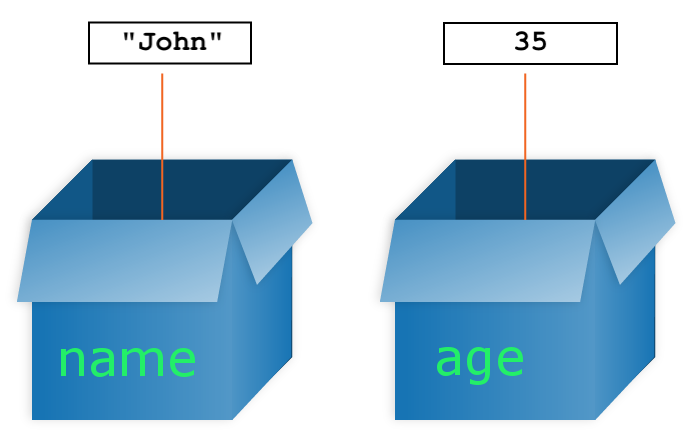
\includegraphics[height=4.25cm]{boxesVariable}
\caption{Zwei Variablen, dargestellt als Behälter mit Namen.\protect\footnotemark.}
\label{figure-variables-boxes}
\end{figure}

\footnotetext{Angepasst von \url{http://www.pyworld.in/Python/pythonVariables.html?i=1}.}

Jeder Behälter in \autoref{figure-variables-boxes} besitzt eine Beschriftung und einen gespeicherten Wert. Der Behälter mit der Beschriftung \lstinline{name} entspricht einer Variablen mit dem Namen \lstinline{name}. Darin wird der Wert \lstinline{"John"} (ein Text) gespeichert. Die andere Variable hat den Namen \lstinline{age} und speichert den Wert \lstinline{35} (eine Zahl).

\begin{definition}[Variable]
Eine Variable ist ein Speicherplatz mit einem Namen. In der Variablen kann ein beliebiger Wert gespeichert werden. Dies geschieht in Python mit einer \textbf{Zuweisung}. Den gespeicherten Wert können wir auch auslesen. Dazu notieren wir den Namen der Variablen. Den Namen einer Variablen können wir selbst wählen.
\end{definition}

\subsection{Was ist ein Wert?}

Computerprogramme verarbeiten Daten. Ein \textbf{Wert} ist eines der grundlegenden Dinge, mit denen ein Programm arbeitet. Die Zahl \lstinline{42} oder der Text \lstinline{"2001: Odyssee im Weltraum"} sind zwei Beispiele für einen Wert. Werte können wir in verschiedene Kategorien aufteilen. \autoref{figure-values-1} zeigt eine Übersicht der bisher kennengelernten Werte. 

\begin{figure}[htb]
\centering
\begin{tikzpicture}[sibling distance=4cm, level distance=1cm, edge from parent/.style = {draw, -latex, thick}]
  	\node {Werte}
    child {	 node[{shape=rectangle, thick, rounded corners, draw, align=center, top color=white, bottom color=blue!20}] (numericvalues) {Zahlenwerte}
    	child {
    		node[{shape=rectangle, thick, rounded corners, draw, align=center, top color=white, bottom color=blue!20}] (integervalues) {ganze Zahlen}
    	}
    	child {
    		node[{shape=rectangle, rounded corners, draw, align=center, top color=white, bottom color=blue!20}] (floatingpointvalues) {Fliesskommazahlen}
    	}
    }
    child { node[{shape=rectangle, thick, rounded corners, draw, align=center, top color=white, bottom color=blue!20}] (textvalues) {Textwerte}
    };
	\node (intexample) [below = 0.1cm and 0cm of integervalues] {z.B.  \lstinline{ -5 } oder \lstinline{ 42}};
	\node (floatexample) [below = 0.1cm and 0cm of floatingpointvalues] {z.B. \lstinline{2.75 } oder \lstinline{ -3.0}};
	\node (textexample) [below right = 0.1cm and -1cm of textvalues] {z.B. \lstinline{"red" } oder \lstinline{ "KSWE"}};
\end{tikzpicture}
\caption{Diese Darstellung ist nicht abschliessend. Es gibt noch mehr Kategorien.}
\label{figure-values-1}
\end{figure}

Einen Wert können wir \textbf{direkt darstellen}, in dem wir den Wert in das Programm eintippen.

\begin{definition}[Literal]
	Eine Zeichenfolge, welche zur direkten Darstellung von Werten benutzt wird, nennen wir Literal.
\end{definition}

\begin{example}
	\lstinline{-5}, \lstinline{42}, 	\lstinline{2.75}, \lstinline{-3.0}, 	\lstinline{"red"} und \lstinline{"KSWE"} sind Beispiele für Literale.
\end{example}

Neben Literalen ist es auch möglich, durch einen \textbf{Funktionsaufruf} einen Wert zu \textbf{erzeugen}.

\begin{example}

\autoref{lst-random-value} und \autoref{lst-sqrt-value} zeigen, wie wir mit einem Funktionsaufruf einen Wert erzeugen. Die Programme beinhalten neben den erzeugten Werten auch Literale (\lstinline{1}, \lstinline{101} und \lstinline{42}). 

\begin{lstlisting}[caption={Erzeugt eine Zufallszahl zwischen $1$ und $100$ und gibt diese dann in der Konsole aus.}, label={lst-random-value}]
import random

zufallszahl = random.randrange(1, 101)
print(zufallszahl)
\end{lstlisting}
	
\begin{lstlisting}[caption={Berechnet die Quadratwurzel aus $42$ und gibt diese dann in der Konsole aus.}, label={lst-sqrt-value}]
import math

quadratwurzel = math.sqrt(42)
print(quadratwurzel)
	\end{lstlisting}
\end{example}

\section{Was ist eine Zuweisung?}

Wir haben mit \lstinline{a = 275} einen neuen Befehl kennengelernt. Der Befehl gehört zur Kategorie \say{Zuweisung} (eng. assignment). \lstinline{a = 275} ist somit ein Beispiel für eine \textbf{Zuweisung}.
$$
\begin{array}[t]{c}
\begin{array}[t]{ccc} 
\underbrace{\textrm{\texttt{a}}}_{\textrm{Variablenname}} & \underbrace{\textrm{\texttt{=}}}_{\textrm{Zuweisungsoperator}} & \underbrace{\textrm{\texttt{275}}}_{\textrm{Wert}}
\end{array} \\
\underbrace{\hspace{6cm}}_{\textrm{Zuweisung}}
\end{array}
$$
Wir können die Zuweisung auch lesen als \say{\lstinline{a} soll $275$ speichern}. Eine Zuweisung erkennen wir am \textbf{Zuweisungsoperator}\footnote{Sie kennen den Begriff bereits aus der Mathematik. Bei der Addition von zwei Zahlen, z.B. $2 + 3$, stellt das \say{Pluszeichen} einen mathematischen Operator dar. Oft wird in der Mathematik auch der Begriff Rechenzeichen verwendet.} (eng. assignment operator). Da das Gleichheitszeichen (\lstinline{=}) in Python für das Speichern von Werten in einer Variablen benutzt wird (und nicht wie in der Mathematik im Sinne einer Gleichung), verwenden wir für das Symbol den Fachbegriff Zuweisungsoperator.

\begin{important}
	Bei einer \textbf{Zuweisung} muss auf der \textbf{linken} Seite des Zuweisungsoperators eine Variable stehen.  
\end{important}

\section{Wo wird der Inhalt einer Variablen gespeichert?}

Eine Variable ist ein Speicherplatz mit einem Namen. Das Computerbauteil, in dem der Speicherplatz für eine Variable reserviert wird, heisst \textbf{Arbeitsspeicher}. Häufig wird das Bauteil auch als \ac{RAM} bezeichnet, da für den Arbeitsspeicher im Computer fast ausschliesslich dieser Speichertyp verwendet wird. Der Arbeitsspeicher für Standardnotebooks ist typischerweise zwischen $\qty{8}{\giga\byte}$ und $\qty{32}{\giga\byte}$ gross. Nur ein \textbf{Teil} davon wird zur Speicherung von Variablen verwendet. 

\section{Welche Variablennamen sind erlaubt?}

Den Namen einer Variablen können Sie fast frei wählen. Sie können Gross- und Kleinbuchstaben verwenden, Ziffern ($0-9$) und den Unterstrich\footnote{Auch Bodenstrich oder Tiefstrich genannt.} (eng. underscore) ($\_$). Es gibt nur sehr wenige Einschränkungen:

\begin{itemize}
\item Der Name darf \textbf{nicht} mit einer \textbf{Ziffer beginnen}.
\item Der Name darf \textbf{nicht} einem Schlüsselwort (eng. keyword) \footnote{Auch reserviertes Wort genannt. Dies sind Wörter, die in Python eine bestimmte Bedeutung haben. Zum Beispiel ist \lstinline{import} ein Schlüsselwort. Schlüsselwörter werden in einer \ac{IDE} meist farblich hervorgehoben.} von Python entsprechen.
\item Der Name darf \textbf{keine} Leerzeichen beinhalten.
\end{itemize}

Die Namen \lstinline{1farbe}, \lstinline{import} und \lstinline{meine Farbe} sind somit \textbf{nicht} erlaubt. \lstinline{farbe1}, \lstinline{warenimport} und \lstinline{meineFarbe} sind hingegen erlaubt.

\begin{important}
Python \textbf{unterscheidet} zwischen Gross- und Kleinbuchstaben. Wir sagen, die Programmiersprache ist \textbf{case sensitive}.
\end{important}

\begin{example}
	Wenn Sie eine Variable \lstinline{tmp}\footnote{Abkürzung für \textbf{t}e\textbf{mp}orary.} verwenden und an einer anderen Stelle \lstinline{TMP} schreiben, dann sind das für Python \textbf{zwei unterschiedliche} Variablen. 
\end{example}

Übrigens: Die korrekte Verwendung der Gross- und Kleinbuchstaben gilt auch für Schlüsselwörter (wie \lstinline{import}).

\section{Wie wählen wir die Variablennamen?}

Eigentlich können wir recht frei einen Namen wählen, zum Beispiel \lstinline{Meine_LiebliNgs_figur} oder \lstinline{birne}. Jedoch \textbf{sollten} wir einen Variablennamen so wählen, dass wir durch den Namen erkennen können, was für ein Wert darin gespeichert ist. Dies entspricht der \textbf{Clean-Code}-Idee.

\begin{cleancode}[Sinnvolle Variablennamen]
Wir wählen \textbf{Variablennamen} so, dass wir möglichst direkt verstehen, was darin gespeichert wird.
\end{cleancode}

\begin{example}
In \autoref{lst-quadrat-var-100} haben wir den Namen \lstinline{a} für die Variable gewählt. Der Name bezeichnet die Seitenlänge des Quadrats. Dies kann als ein sinnvoller Name betrachtet werden, da die Seitenlänge eines Quadrats typischerweise in der Geometrie mit $a$ bezeichnet wird. Ausserdem wird das Programm unter dem Namen \graybgtexttt{quadrat\_var.py} gespeichert. Daraus ist ersichtlich, dass es sich um die Seitenlänge handeln muss. Wir können es auch noch expliziter machen und den Namen \lstinline{seitenlänge} verwenden.\\
Ein schlechter Name wäre \lstinline{apfel}. Dieser Name sorgt für Verwirrung. Geht es hier um Obst? Was wird in einer Variablen mit dem Namen \lstinline{apfel} gespeichert? Warum eine Zahl? Sollte es nicht eine Apfelsorte sein?
\end{example}

\begin{cleancode}[Snake Case]
In Python ist es üblich, für Variablennamen \textbf{nur} Kleinbuchstaben zu verwenden. Besteht der Name aus mehreren Wörtern, dann \say{trennen} wir diese Wörter durch einen Unterstrich ($\_$). Diese Schreibweise wird Snake Case genannt. 
\end{cleancode}

\begin{example}
	Die Variablennamen \lstinline{meine_farbe}, \lstinline{zahl_1} oder \lstinline{temperatur_in_celsius} sind in Snake Case notiert.
\end{example}

\begin{hinweis}
	Andere Programmiersprachen empfehlen andere Schreibweisen für Variablennamen. \autoref{figure-naming-conventions} zeigt auf humorvolle Art die gebräuchlichsten Schreibweisen.	
\end{hinweis}

\begin{figure}[htb]
	\centering
	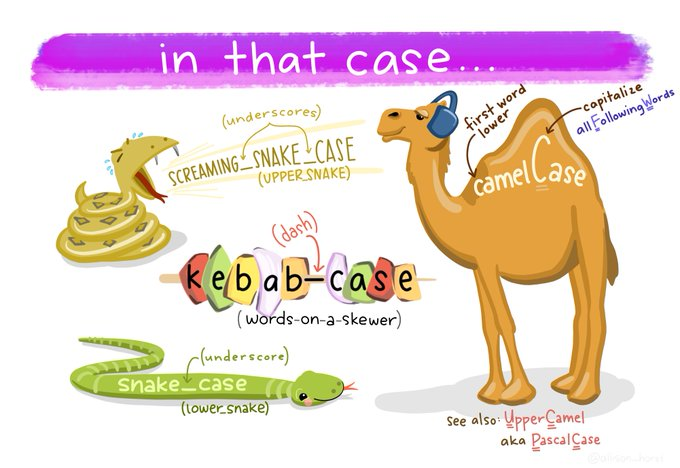
\includegraphics[height=8cm]{naming_conventions}
	\caption{In Python ist \protect\say{Snake Case} üblich.}
	\label{figure-naming-conventions}
\end{figure}


\section{Wie benutzen wir den Inhalt einer Variablen?}

Wir können jederzeit den Inhalt einer Variablen benutzen, in dem wir den entsprechenden \textbf{Variablennamen} notieren. Python ersetzt dann während der Ausführung den Variablennamen durch den gespeicherten Inhalt. Wir sagen, die Variable wird \textbf{ausgelesen}.

\begin{example}
	Im Programm aus \autoref{lst-quadrat-var-100} wird der Inhalt der Variablen \lstinline{a} an vier Stellen benutzt. In Zeile vier wird für den Funktionsaufruf die Variable als Argument verwendet. Die Variable wird während der Ausführung durch die gespeicherte Zahl ($100$) ersetzt. Dies wiederholt sich für die Zeilen sechs, acht und zehn.
\end{example}

\begin{important}
	Das Auslesen einer Variable löscht den gespeicherten Inhalt der Variable \textbf{nicht}.
\end{important}

\begin{hinweis}
	Falls beim Auslesen die passende Variable nicht existiert (da zum Beispiel vorher kein Wert darin gespeichert wurde), dann gibt es eine \textbf{Fehlermeldung}. Typischerweise wird ein \texttt{NameError} erzeugt.
\end{hinweis}


\section{Aufgaben}

In den folgenden Aufgaben setzen Sie sich mit Variablen auseinander.

\subsection{Aufgabe 1}

Entscheiden Sie für \textbf{jeden} Variablennamen, ob es sich um einen gültigen Namen handelt oder nicht. In dieser Aufgabe spielt der Clean-Code-Gedanke keine Rolle. Es geht nur darum, ob der Name gültig ist. Falls es sich um einen ungültigen Namen handelt, dann markieren Sie die ungültigen Zeichen. Ist es ein gültiger Name, dann markieren Sie dies mit \checkmark.

\begin{multicols}{2}
\begin{enumerate}
\item \lstinline{Monty Python}
\item \lstinline{monty python}
\item \lstinline{monty_python}
\item \lstinline{0ahnung}
\item \lstinline{s109}
\item \lstinline{meine_lieblingsfarbe}
\end{enumerate}
\end{multicols}

\subsection{Aufgabe 2}

\begin{enumerate}

\item Es ist 13:37:42 Uhr. Die Anzahl der Stunden, die Anzahl der Minuten und die Anzahl der Sekunden soll jeweils in einer Variablen gespeichert werden. Notieren Sie das passende Programm und beachten Sie die \textbf{Clean-Code-Regeln} bzgl. Variablennamen.
\fillwithgrid{0.75in}

\item Die Temperatur beträgt \qty{27}{\degreeCelsius}. Notieren Sie ein Programm, welches diese Temperatur in einer Variablen speichert. Verwenden Sie einen sinnvollen Namen.
\fillwithgrid{0.25in}

\item Die Latenz beträgt \qty{21}{\ms}. Notieren Sie ein Programm, welches diese Latenz in einer Variablen speichert. Verwenden Sie einen sinnvollen Namen.
\fillwithgrid{0.25in}

\end{enumerate}

\subsection{Aufgabe 3}

Studieren Sie das \autoref{lst-rhombus}. Schreiben Sie das Programm so um, dass drei Variablen mit sinnvollen Namen benutzt werden. Definieren Sie die Variablen nach der \lstinline{import}-Anweisung.

\begin{important}
Jeder \textbf{Wert} (z.B. \lstinline{100} in \lstinline{turtle.fd(100)}) kann durch eine \textbf{Variable} \say{ersetzt} werden, die den gleichen Wert speichert (z.B. \lstinline{a = 100} und dann \lstinline{turtle.fd(a)}).
\end{important}

\begin{minipage}{0.35\textwidth}
\centering
\begin{lstlisting}[caption={Ein Rhombus.}, label={lst-rhombus}]
import turtle

turtle.fd(100)
turtle.lt(120)
turtle.fd(100)
turtle.lt(60)
turtle.fd(100)
turtle.lt(120)
turtle.fd(100)
turtle.lt(60)
turtle.done()
\end{lstlisting}
\end{minipage}
\hfill
\begin{minipage}{0.55\textwidth}
\centering
\fillwithgrid{2.75in}
\end{minipage}